%\section{Computing Continuum}
%\label{sec:example}
%
%%Herein we will discuss the challenges of developing a mobile application that exploits the computing continuum, as well as present a running example that will be used throughout the rest of the paper to exemplify our work.
%
%As previously stated, the continuum enables the convergence of many heterogeneous infrastructures, from cloud-hosted virtual machines down to mobile devices. Given that the two fundamental elements of computation are data and behavior, the first major challenge of developing an application that exploits the computing continuum consists in \emph{deciding where in the continuum the data and the behavior should be deployed}. This decision needs to be informed by the profound heterogeneity that exists between the different infrastructures that constitute the continuum. 
%
%Amongst other things one must take into account important QoS aspects, such as availability and latency, as discussed in Section~\ref{sec:intro}. Let us focus, for example, on a continuum that comprises a cloud-based solution, an edge-based infrastructure, and a mobile device. Data and behavior that are deployed to cloud solutions will benefit from high availability, at the cost of introducing higher latency; while data and behavior deployed to an edge-based infrastructure will benefit from a much lower latency, at the cost of having a lower availability as well. A third possibility would be to deploy the data and the behavior exclusively to the mobile device; however, this could lead to important battery drains (see Section~\ref{sec:evaluation}), not to mention other limitations. Balancing these trade-offs at design time can be difficult. The challenge is, therefore, to allow applications to dynamically, and opportunistically, decide where the data and the behavior should be deployed and executed. 
%
%If we focus on behavior, it is common to distinguish between stateful and stateless computation. The main distinguishing factor between stateful and stateless components is that the latter do not produce side-effects, and that their outputs depend solely on their inputs. If we focus on data, it is common to distinguish between mutable and immutable data. While mutable data can be modified after its creation, the same is not true for immutable data. In components that adopt immutable data, the data is initialized once and for all at deployment time.
%
%As we shall discuss in Section~\ref{sec:proposal}, it is our view that the computing continuum should focus on stateless computation with immutable data. Stateless computation with immutable data is much easier to replicate (and test) across the continuum, since no data synchronization is required and any data needed by the computation can be obtained at deployment time. Nevertheless, stateful computation and mutable data cannot always be excluded entirely from modern applications. For these cases we envision a mixed solution in which traditional cloud-based resources are adopted alongside the continuum. 
%
%Developing applications in the computing continuum also poses other important challenges. For example, when selecting where a certain computation should be achieved, we need to take into account important \emph{security} aspects, such as \emph{authorization}, \emph{confidentiality}, and \emph{integrity}. Also, deployment and execution in the continuum will need \emph{tool} support, e.g., for performing \emph{integration tests}, \emph{runtime monitoring and adaptation}, etc. 
%
%Although these challenges are interesting, and important research endeavors in themselves, in this paper we focus on establishing the basis upon which the computing continuum can develop. In particular, we focus on achieving (i) the dynamic and automatic deployment of computation by part of the infrastructures that constitute the continuum, and (ii) the opportunistic selection of where to execute the computation.

%END OF PREVIOUS CONTINUUM

%REVISED CONTINUUM

\section{The Continuum Model}\label{sec:continuum}
%
%\begin{figure}[tbp]
%	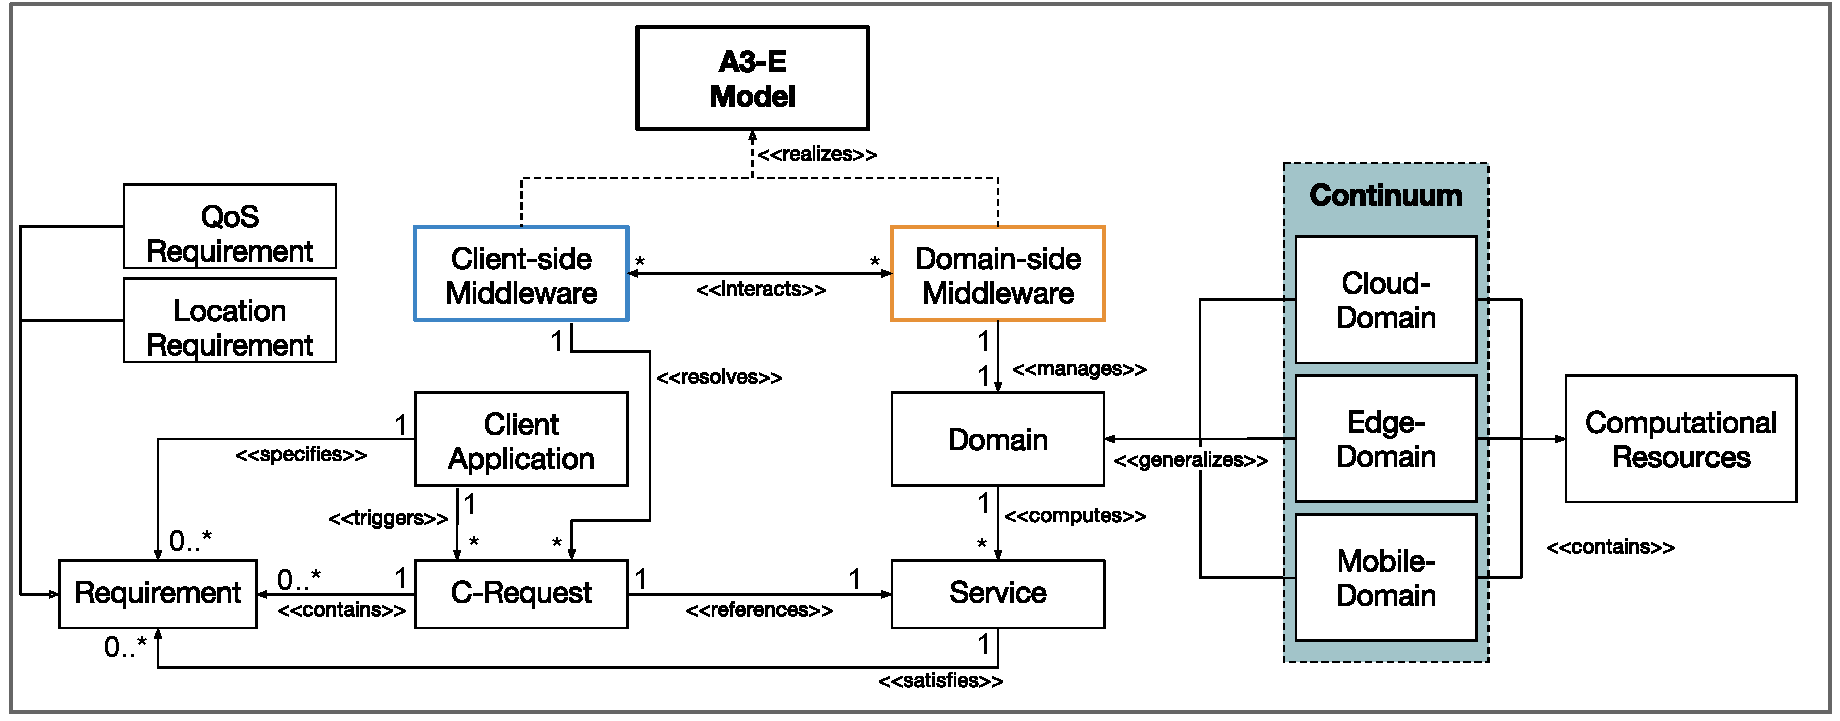
\includegraphics[width=1\textwidth]{figs/A3-E-model.pdf}
%	\caption{The Continuum Model.}
%	\label{fig:Continuum-model}
%\end{figure}

%The \textit{Continuum model}, depicted in Figure~\ref{fig:Continuum-model}, defines the actors and mechanisms involved in the realization of the mobile-edge-cloud continuum.

%Domain formalization
%Application Requirements
%Service SLA
%Service Life-cycle

\subsection{Physical Model}

%Although the continuum can hypothetically support any number of heterogeneous infrastructures, this paper focuses on three domains. The \texttt{mobile domain} is deployed to the client's mobile device, and provides local stateless computation (while enabling device-to-device collaboration through distributed mobile domains --i.e., by allowing a client to call a microservice deployed on another mobile device-- is surely interesting, for now we consider it part of our future work). The \texttt{edge domains} refer to edge-based infrastructure that can be deployed to a local server (local-edge domain) or to cellular stations (mobile-edge domain). Finally, the \texttt{cloud domain} refers to a cloud-based solution such to AWS Lambda.

%The continuum is composed of computational resources from cloud, edge, and mobile computing devices. 
%
%Cloud datacenters count with virtually unlimited computational resources needed to cope with the aggregated demand from a wide coverage area. Edge nodes~\cite{}, in contrast, are limited in computational resources, but cover a much narrower area with lower aggregated demand. 
%
%Cloud datacenters are reachable through multiple hops of network, including the Internet backbone. Edge nodes, in turn, are ideally placed a few hops away from clients to minimize network latency and jitter. 

%TODO [Martin] I've slightly changed this and next paragraph to be compliant with the ETSI standard
In our formulation, edge nodes are distinguished after the networking technology they use: \textit{mobile edge} hosts (in the context of Multi-Access Edge Computing or MEC~\cite{etsimec16,ahmed2016isco}) integrate with cellular network infrastructure (e.g., a 5G base station), whereas \textit{local edge} ones integrate with local area network infrastructure (e.g., an access point). Also, we assume that cloud and edge providers may be different from each other, and that communication among heterogeneous (mobile) edge systems~\cite{etsimec16} may not be feasible.% and unable to coordinate the allocation of resources.

%Later on, this heterogeneity is addressed with variations of the proposed service life-cycle management.

Mobile devices play two roles, namely clients and potential providers of continuum services. The motivation for including mobile devices' own  resources in the model is threefold: (i) the substantial increase in computational capacity exhibited by modern devices; (ii) the compatibility of these devices with the computation of continuum microservices (see Section~\ref{sec:application_model}); and (iii) to give mobile applications a zero network latency and highly available alternative to cloud and edge providers. 

%TODO fix Figure X
%Figure X~\ref{fig:topology} illustrates a topology composed of cloud, mobile-edge, local-edge, and mobile \textit{domains}. 
%Throughout this paper, we refer to \textit{cloud}, \textit{edge}, and \textit{mobile} \textit{domains}. 
Each part of the continuum topology (cloud, mobile-edge, local-edge, and mobile) is composed of domains.
A domain yields a common  abstraction for the heterogeneous compute, storage and network resources (e.g., server(s), virtual machine(s), container(s), memory, CPU, storage, etc.) composing the continuum. In the particular case of MEC, the term \textit{domain} extends the one provided by ETSI for a \textit{mobile edge host}~\cite{etsimec16}.



%constituents of the continuum. Indeed, it hides the fact that they make use of heterogeneous \textit{computational resources} (e.g., server(s), virtual machine(s), container(s), memory, CPU, storage, etc.) and networking infrastructures (e.g., access points, radio access networks, etc.). 

%Examples of A3-E domains are \textit{cloud domains}, i.e., cloud-based FaaS platforms covering a specific geographical region (e.g., AWS Lambda\footnote{\url{https://aws.amazon.com/lambda}} in Europe); \textit{edge domains}, representing local-edge (e.g., domestic servers or within an office building) and mobile-edge sites (e.g., servers at cellular base stations~\cite{beck2014mobile}); and \textit{mobile domain} representing a client device's own resources.

%TODO


%Whilst cloud and edge resources are shared among different applications and managed by cloud/edge providers, mobile device resources are exclusively employed by local applications. 

\subsection{Application Model}\label{sec:application_model}

\begin{figure}[tbp]
	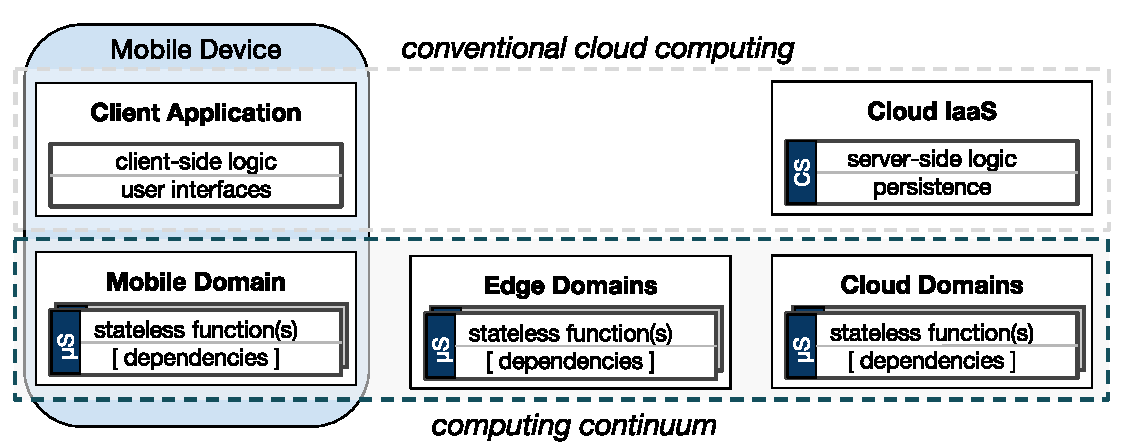
\includegraphics[width=0.85\textwidth]{figs/Continuum-arch}
	\setlength{\belowcaptionskip}{-10pt}
	\caption{The high level architecture of a mobile application exploiting both the computing continuum -- by means of $\mu$-services ($\mu$S) provided by mobile, edge, and cloud domains -- and conventional mobile/cloud computing -- by means of local computation and cloud services (CS).}
	\label{fig:Continuum-arch}
\end{figure}

On top of the physical model, we propose an \textit{application model} in which stateless components and immutable data composing \textit{continuum services} are dynamically placed to mobile, edge, and cloud,
whilst 
stateful components are deployed to cloud datacenters or the client device itself based on design-time decision.

Continuum services consist of a set of artifacts that fulfill a given functionality. In particular, these artifacts can refer to: (i) stateless function(s) (e.g., a Java compiled class); (ii) immutable data (e.g., a trained neural network model); and (iii) other dependencies (e.g., software libraries).

A priori, continuum services are portable, unless they require capabilities that can not be met by specific domains. Like cloud and edge domains, mobile domains also expose functionality by means of a well-known interface --- for the sake of consistency, the service abstraction is employed within all domains.

The proposed service model enforces data consistency and allows multiple service instances to coexist along the continuum. Also, service instances may be deployed and undeployed independently without the need for state migration, favoring the seamlessly transition from one service provider to the other. The latter is particularly important to cope with the mobility of clients. 

Continuum services are also aligned with the \textit{Function-as-a-Service} (FaaS) execution model~\cite{MateosFaaster17}. FaaS has been proposed as an alternative cloud paradigm in which business functionality is provided without pre-allocating computational resources. Instead, shared resources (e.g. containers) are used to provision and execute functions on demand, in only a few milliseconds. 

Services implemented after the FaaS model are \textit{microservices}\footnote{Hereafter referred as $\mu$-service}~\cite{lewis2014microservices}, as they are small, modular, communicate with lightweight mechanisms (often through an HTTP RESTful API) and are independently deployable by fully automated machinery. Note that our approach targets application-level functions, whereas Virtualized Network Functions (VNFs~\cite{etsimec16}) are considered as a part of the underlying infrastructure.

%This requires to support FaaS not only at cloud level, but also to bring it to (mobile) edge platforms~\cite{etsimec16}. 



As state is a fundamental aspect of many applications, we propose that mobile devices and, for most cases, cloud datacenters should remain responsible for stateful components such as persistence. This choice prevents the consistency problems (and the corresponding complexity of potential solutions) that would arise if databases were deployed to finely distributed edge nodes. %This decision is also aligned with the limitations in computational resources of edge nodes. %Indeed, the deployment of components like databases to the edge would be unrealistic for large scale applications.

%TODO: make it more general, as some applications may have local persistence and u-services may also deal with business logic
Figure~\ref{fig:Continuum-arch} illustrates the architecture overview of a continuum application. The client-side application comprises \texttt{client-side logic}, \textit{local persistence}, and \texttt{user interface} components, whereas the cloud infrastructure comprises \texttt{server-side logic} and \texttt{persistence} components. Continuum $\mu$-services are responsible for stateless computation opportunistically deployed to different domains.

\subsection{Life-cycle Management Challenges}

% [Danilo] It's been really hard to change the formulation without falling in the trap of not been objective. For me, Awareness is mostly about letting domains to know *when* to allocate resources and to let clients to know *which* domains can be chosen. Please let me know if you have insights about it. For sure I agree to make the formal part easier to digest, but it wouldn't change the focus on allocation/placement. 

The management of continuum services life-cycle is focused on two conflicting goals: i) the satisfaction of application requirements (e.g., maximum service latency, battery consumption, availability); and ii) the optimization of resources allocated for the applications. 

Dynamicity is a fundamental aspect in the continuum as mobile clients are likely to enter and exit areas covered by distinct edge domains. The aggregated demand served by cloud domains should also expect considerable variations. In any case, it may be unfeasible to predict when and how intense the demand from different applications and users will be. 

From the providers' perspective, an optimal allocation of its (virtualized) resources corresponds to the minimum number of $\mu$-service instances that must be allocated by each of its domains to cope with the SLA of each provided $\mu$-service. To be efficient, the allocation of resources should be able to mimic the corresponding fluctuations of demand, i.e., to be highly responsive. For that matter, it is important that the mechanisms governing resource allocation from each domain to be \textit{aware} of actual and potential demand for its provided $\mu$-services. 

% (e.g., maximum service latency, simultaneous request threshold, etc). 


%Even if emerging network technologies could be employed to route traffic from one base station to the other, continuum $\mu$-services implemented after the FaaS model are ephemeral (they may even last for only one invocation), stateless, and scaled as needed~\cite{Roberts:2016}. 

%In FaaS, functions are ephemeral (they may even last for only one invocation), stateless, and scaled as needed~\cite{Roberts:2016}. 

To better express this problem, let's consider the set of $\mu$-services $S = \{s_j \mid j = 0,1,...,J\}$.
%In turn, $F_i = \{f_{i,j}\}_j$ defines the set of instances of $s_i$, with $0 \le j \le n_i$.
%Instances for each $\mu$-service are defined by the set $F_i = \{f_{i,j}\}_j$, with $0 \le j \le n_i$.
Vector $\bar{c} = (c_1, ..., c_J)$ holds the number of instances for all $\mu$-services. Each instance is bound to a container; resources allocated to each container 
%Each $s_j \in S$ has a corresponding set of instances $F_j = \{f_{j,i} \mid i = 0,1,...,I_j\}$, where each instance is bound to a container. 
(e.g., CPU and memory) are considered fixed and equal for all $\mu$-services, coherently to the architecture of FaaS frameworks such as OpenWhisk~\cite{OpenWhisk}.

Now let's consider that each provided $\mu$-service $s_i \in S$ is bound to an SLA specifying its maximum service delay $\Delta_j$ and the maximum/minimum number of instances $Imin_{j}/Imax_{j}$, so that $\forall s_j \in S, Imin_j \le c_j \le Imax_j$. %, and a relative priority $p_i$. 
Given the fluctuations in the workload and the perceived delay $\tau_j$ of each service $s_j \in S$, the aim of a \textit{domain manager} is to assure that $\forall s_j \in S, \tau_j \le \Delta_j$.

Last but not least, if we consider a plethora of disjoint domains able to host the execution of $\mu$-services, each domain must be able to autonomously manage operational aspects such as the \textit{download and deployment} of $\mu$-services from new applications. 

%Also, each instance $f_{ij} \in F_i$ is bound to a single core container with fixed memory and storage. Considering that CPU is a scarcer resource, we may assume, without loss of generality, that the number of $\mu$-instances per domain is limited by the amount of CPU cores available ($|C|$) in its pool of resources, i.e., that $\sum_{i=1}^{m} k_i \le |C|$.

%Furthermore, as the demand for different services is expected to change over time, unless $\forall S_i \in S, U_i = U_i$, idle resources may be employed to reduce $\delta_i$ according to $P_i$.

From the client's viewpoint, the challenges for the materialization of the continuum are mainly twofold: i) surrogate edge domains may need to be dynamically discovered; ii) the client may need to choose among different domains able to provide similar $\mu$-services.

For a continuum application, an optimal domain selection is the one that, given a set of requirements and the perceived QoS of different services, satisfies the multi-criteria decision of which provider to be employed. Moreover, since continuum $\mu$-services are modular and independently deployed, it consists of individual decisions regarding each $\mu$-service consumed by the application.

To better express the client-side selection, let's extend the previous formulation by considering a set of independent provider domains $D = \{d_p \mid p = 1,2,...,P\}$. Each domain $d_p \in D$ provides a set of $\mu$-services $S_{p} = \{s_{p,i} \mid i =  0, 1, ..., I_p\}$. In turn, a continuum application $CA_x$ relies on the set of $\mu$-services $S_x = \{s_a \mid a = 1,2,...,A\}$, so that $\forall s_a \in S_x$, there is at least one provider domain offering that $\mu$-service, that is, $\forall s_a \in S_x, \exists\ s_{p,i} \in \bigcup_{p=1}^{|P|} S_p \wedge s_{p,i} = s_a$. 

Now let's consider that each $s_a \in S_x$ is bound to a set of required QoS attributes $QoS_a = \{qa_u \mid u = 0, 1, ..., U\}$ and that each $qa_u \in QoS_a$ is represented by a tuple $(constraint_u, weigth_u)$ respectively defining the an expression (e.g. response time < 300ms) and weight for that attribute. For each $qa_u \in QoS_a$, $actual_{p,a,u}$ defines the value for that QoS attribute as perceived by the client. It follows that, for each $s_a \in S_x$ from application $CA_x$, the aim of the \textit{mobile middleware} is to select the domain $d_p \in D$ 
%best satisfying the set of attributes in $QoS_o$, i.e., 
that maximizes the utility function $U(p) = \sum_{u=1}^{U} weigth_u * actual_{p,a,u}$, provided that $\forall qa_u \in QoS_a, actual_{p,a,u} \vdash constraint_u$.

%service latency and cost as our requirements. From the client viewpoint, latency can be refined into network and service latency, with cloud providers exhibiting highest network latency and lowest service latency due to more powerful computational power; edge providers exhibiting low network latency and higher service latency; and finally the local mobile environment exhibiting zero network latency and the highest service latency due to more limited computational power. Service cost, in turn, is lower in the cloud than in the edge and null in the mobile environment. Given the relative importance of each attribute, the aim of the provider selection is to 


%The life-cycle management is therefore dual: it comprises the provider-side allocation of service instances at each domain; and it also encompasses the client-side decision of which domain must be selected for each continuum $\mu$-service.

\subsection{Running Example}
\label{sub:example}

\begin{figure}[tbp]
	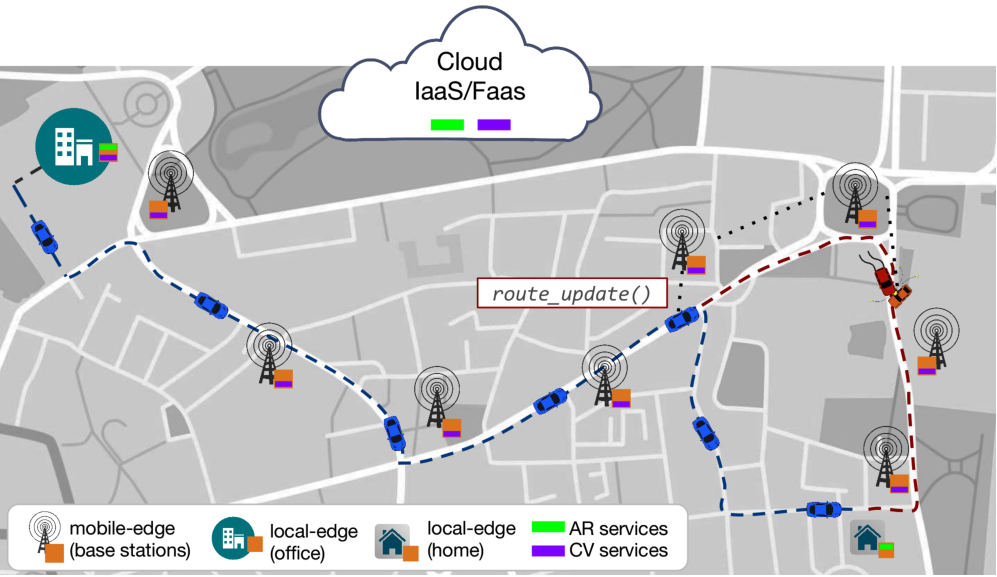
\includegraphics[width=0.7\textwidth]{figs/Continuum-Scenario}
	\setlength{\belowcaptionskip}{-8pt}
	\caption{Heterogeneous applications such as Augmented Reality and Mobile Games (MG) rely on $\mu$-services deployed along the compute continuum (mobile, mobile-edge, local-edge, and mobile).}
	\label{fig:continuum-scenario}
\end{figure}

%Figure~\ref{fig:continuum-scenario} shows a complete example scenario involving different applications that rely on computation executed in the cloud, edge, or in the user's own devices.

We illustrate the continuum with an example scenario involving different applications that rely on computation executed in the cloud, edge, or in the user's own device.

First, let us consider an Augmented Reality (AR)~\cite{GarrigaMendonca2017} application employed by our user to 
explore the points of interest (POI) in the touristic areas from the city she is currently visiting.
%craft virtual 3D objects that are added to her \textit{smart glasses} as part of her work. 
This real-time application involves heavyweight image processing for the \textit{extraction of features} from the captured scenes, as well as a trained neural network model to \textit{match features} from an extensive object catalog.

Two continuum $\mu$-services are modeled after each task: one relies on a image processing library and a trained model, the other on a feature-based object catalog. Client-side logic is responsible for capturing scenes from the glasses' camera and updating the 3D virtual object in the scene rendered by the smart glasses.

Despite the capacity of existing smart devices (e.g., Glass~\footnote{https://x.company/glass/}) in hosting a plethora of applications, the user may experience functional and non-functional degradation (e.g., reduced object catalog, battery drain, etc). With the offloading of the aforementioned tasks to a server, the user can enjoy an improved Quality-of-Experience with the AR application.

%avoid recharging her glasses and improve productivity. 

To support this and other applications, mobile-edge servers were deployed to the base stations covering touristic areas. Their additional storage allows a larger set of objects to be recognized, thanks to a more completely trained model. Variations in the workload are handled with a fast instantiation of $\mu$-services, which must consider other applications relying on the same servers.

%In contrast, the network latency to cloud servers may be prohibitive for this real-time application. The decision of which continuum provider to employ must be informed by the application requirements and the Quality-of-Service (QoS) of each alternative. 

After her expedition, our user calls for an autonomous vehicle (AV) to drive her back to her hotel. During the way, she starts editing the pictures taken during the tour. To reduce processing time and avoid battery drain, the AV features a local-edge server that provides a catalog of $\mu$-services for image processing. Meanwhile, the vehicle makes use of a \textit{route planning} $\mu$-service
%deployed at mobile-edge servers located at cellular base stations 
to receive updates about the best plan to reach our user's destination. Since latency is not a main requirement, the latter is served by a cloud provider whenever the AV's local-edge server is unavailable. 

%Additionally, it relies on low-latency services to become aware of sudden events like accidents.

%To support the AV, two continuum $\mu$-services are envisioned: the \textit{route planning}, which relies on a traffic dataset and a routing software and can cope with higher latency, and the \textit{incident notification}, which relies on low-latency communication between vehicles and mobile-edge base stations to forward incident events received by that base-station.

%TODO: the incident notification is not consistent with our service model; either remove the AV example or find a different kind of low-latency service (e.g., augmented reality of what is seen from inside the car?)
%[Danilo] What about web sockets? Or push-notification? 

%within milliseconds the vehicle can become aware of to adjust its routes to avoid heavy traffic. In particular, let's say that a new path consists of residential streets with data services only (without mobile-edge coverage). The AV continues to fetch updates, which are now served by a cloud provider. The additional network latency is partially compensated with the low speed limit of the residential area.

%During our user's journey home, her AV passes by a touristic region. The mobile-edge domains covering this area provides continuum $\mu$-services to be consumed by an AR application for tourists. These services share computational resources with those of AVs passing by the same area, as well as any other continuum $\mu$-services that happens to be provided by those mobile-edge domains.

%Due to resource limitation, each mobile-edge domain must employ mechanisms to efficiently manage its resources and assure that competing $\mu$-services are best provided according to their Service Level Agreement (SLA). In our example, the AV's \textit{incident notification} $\mu$-services is likely to enjoy a higher priority regarding the AR's $\mu$-services due to the criticality of the former.

Finally at her hotel room, our user 
%can start using her domestic local-edge. She 
decides to enjoy a Mobile Game (MG) application. The MG consists of client-side logic and user interfaces (e.g., controllers and views of an MVC\footnote{Model-View-Controller architectural pattern}). In particular, the game model features complex calculations that pose a burden to her mobile device's CPU. 
%The application consists of for processing the game state, which must be passed as a parameter in conjunction with game events (e.g., user inputs). 

Supporting guest applications, the hotel is equipped with a local-edge server. The latter identifies the MG application and, upon download and installation, starts providing the $\mu$-services for processing the game state, which must be passed as a parameter in conjunction with game events (e.g., user inputs). Last but not least, conventional cloud services provide stateful server-side logic (e.g. authentication, business logic) and persistence (e.g., player scores).  

%This latter scenario exploits different parts of the continuum. A domestic local-edge domain must identify, fetch, and deploy the corresponding $\mu$-services. Meanwhile and to assure a high availability, the mobile domain remains responsible for the provisioning of these $\mu$-services. Finally, cloud domains complement the possible alternatives for hosting the $\mu$-services and mitigating battery drain, but network latency must be taken into account.

%Traditional cloud resources are employed as a reliable alternative to edge-based computation. Similarly, local services are employed as alternatives to edge services until they have been acquired and made available by a local-edge server. Whilst the transition between mobile-edge and cloud is transparent, the use of local-edge services involves mutual client-server awareness.


%TODO [Danilo] better in proposal
%Upon installation, the local-edge server becomes aware of a new continuum-compliant application and, while the app continues to run locally on her device, it proceeds to setup the services needed to allow the application to offload some of the computation. Once the setup is complete, the application autonomously starts using the edge services with the purpose of preserving the device's resources. Not only does the game's performance improve, battery consumption is also reduced.  




